\chapter{Conception g\'enerale du projet}

\section{Introduction}
Ce chapitre est consacr\'e \`a la conception g\'en\'erale du projet. Apr\`es la d\'efinition des besoins fonctionnels et non fonctionnels, nous allons passer \`a expliquer l'architecture globale du syst\`eme qui repr\'esente une vue g\'en\'erale de notre solution.

\section{Conception g\'en\'erale}


Cette partie se base sur la conception globale de l'architecture fonctionnelle de notre projet. Effectivement, elle explique les composants de notre syst\`eme ainsi la communication entre eux.

\subsection{Architecture globale du syst\`eme}

L'architecture de notre syst\`eme est compose par:

\begin{figure}[h]
	\center{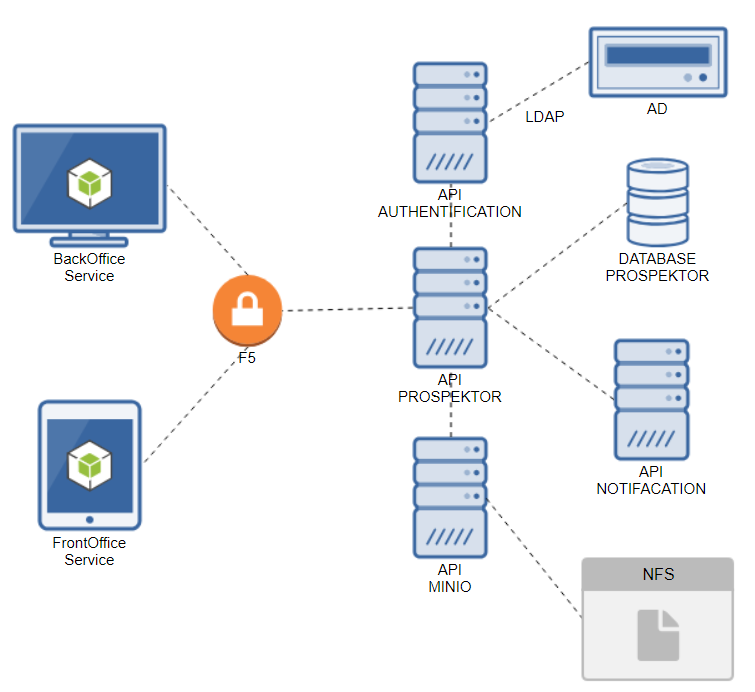
\includegraphics[width=\textwidth]{Figures/architecture.PNG}}
	\caption{\label{fig:my-label} Architecture du syst\`eme}
\end{figure}

\begin{itemize}
\item \textbf{F5 VPN} : utilise le protocole Secure Sockets Layer, une technologie d'authentification et de cryptage int\'egr\'ee \`a chaque navigateur Web, pour cr\'eer une connexion s\'ecuris\'ee et crypt\'ee sur un r\'eseau moins s\'ecuris\'e, comme Internet.
\item \textbf{MINIO} : vous permet d'utiliser un seul \gls{NAS} (comme \gls{NFS}, GlusterFS et d'autres syst\`emes de fichiers distribu\'es) en tant que syst\`eme de stockage pour plusieurs serveurs MinIO. La synchronisation entre les serveurs MinIO est prise en charge par la conception.
\item \gls{AD} est un syst\`eme bas\'e sur une base de donn\'ees qui fournit une authentification, un annuaire, une strat\'egie et d'autres services dans un environnement Windows.
\item \gls{LDAP} est un protocole d'application permettant d'interroger et de modifier des \'el\'ements dans des fournisseurs de services d'annuaire tels qu'Active Directory, qui prend en charge une forme LDAP.
\item \gls{NFS}, litt\'eralement syst\`eme de fichiers en r\'eseau, est \`a l'origine un protocole qui permet \`a un ordinateur d'acc\'eder via un r\'eseau \`a des fichiers distants.
\end{itemize}

\subsection{Architecture applicative} 

D'apr\`es l'architecture globale du syst\`eme, on constat qu'elle est composs\'e par deux parties :

\begin{itemize}
\item \textbf{Partie backend :} qui se repr\'esente par l'API prospektor, est la partie serveur ou partie logique m\'etier.
\item \textbf{Partie frontend :} qui repr\'esente la partie client ou partie interface.\\
Dans notre projet, elle se d\'ecompose par deux parties :
\begin{itemize}
\item Une application de \textbf{back-office} comprend le logiciel utilis\'e par une organisation pour administrer des op\'erations qui ne sont li\'ees \`a aucun effort de vente directe et \`a des interfaces qui ne sont pas vues par les consommateurs.
\item En revanche, une application de type \textbf{front-office} serait une interface client facilitant la vente ou le traitement d'une transaction.
\end{itemize}
\end{itemize}



\subsubsection{Cas g\'en\'eral pour le backend}
Pour les services Backend le choix de l'architecture applicative suit une d\'ecomposition en trois couches (3-tiers) :
\begin{itemize}
\item Couche DAO : c'est la couche d'accd\`es aux donn\'ees persistant dans la SGBD.
\item Couche Services : impl\'emente la logique m\'etier du service, et les diff\'erentes rd\`egles de gestion qui repr\'esentent les fonctionnalit\'es du service.
\item Couche API : il permet l'encapsulation des diff\'erents services dans une API RESTfull et fournit les contr\^oleurs l'accd\`es \`a ces services.
\end{itemize}

\begin{figure}[H]
	\center{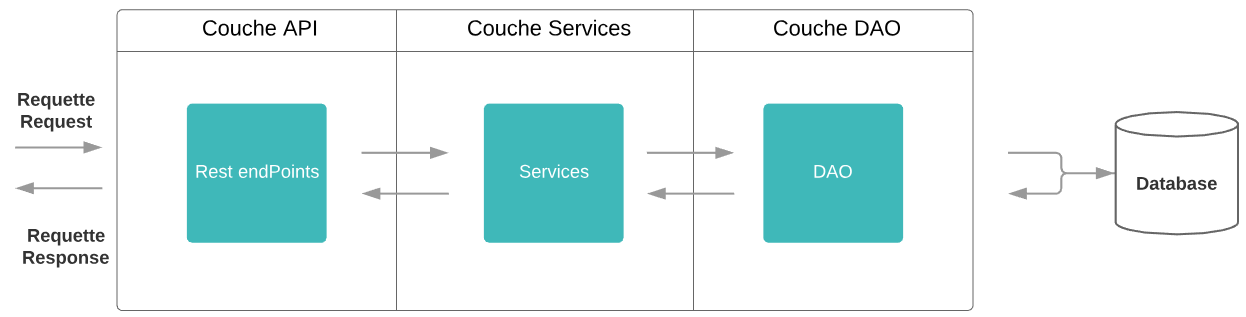
\includegraphics[width=\textwidth]{Figures/backend.PNG}}
	\caption{\label{fig:my-label} Architecture 3-tiers}
\end{figure}

On a aussi impl\'emente l'architecture \gls{MVC} qui signifie  Mod\`ele, Vue et Contr\^oleur. MVC s\'epare les applications en trois composants : 

\begin{itemize}
\item \textbf{Mod\`ele} : Repr\'esentations de mod\`ele sous forme de donn\'ees et de logique applicative. Il contient les donn\'ees de l'application. Les objets de mod\`ele r\'ecup\`erent et stockent l'\'etat du mod\`ele dans une base de donn\'ees.

\item \textbf{View} : View est une interface utilisateur. Visualisez les donn\'ees d'affichage en utilisant le mod\`ele pour l'utilisateur et leur permettre \'egalement de modifier les donn\'ees.

\item \textbf{Contr\^oleur} : le contr\^oleur g\`ere la demande de l'utilisateur. En r\`egle g\'en\'erale, l'utilisateur interagit avec View, ce qui d\'eclenche \`a son tour la demande d'URL appropri\'ee. Cette demande sera g\'er\'ee par un contr\^oleur. Le contr\^oleur rend le appropri\'e
afficher avec les donn\'ees du mod\`ele en r\'eponse.
\end{itemize}

\begin{figure}[H]
	\center{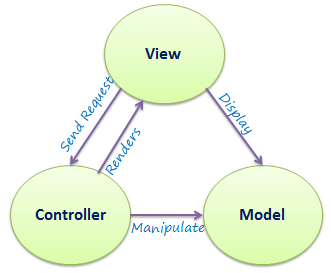
\includegraphics[width=0.7\textwidth]{Figures/mvc.PNG}}
	\caption{\label{fig:my-label} Architecture MVC}
\end{figure}

On obtient comme architecture final pour le cot\'e backend la figure suivante :


\begin{figure}[H]
	\center{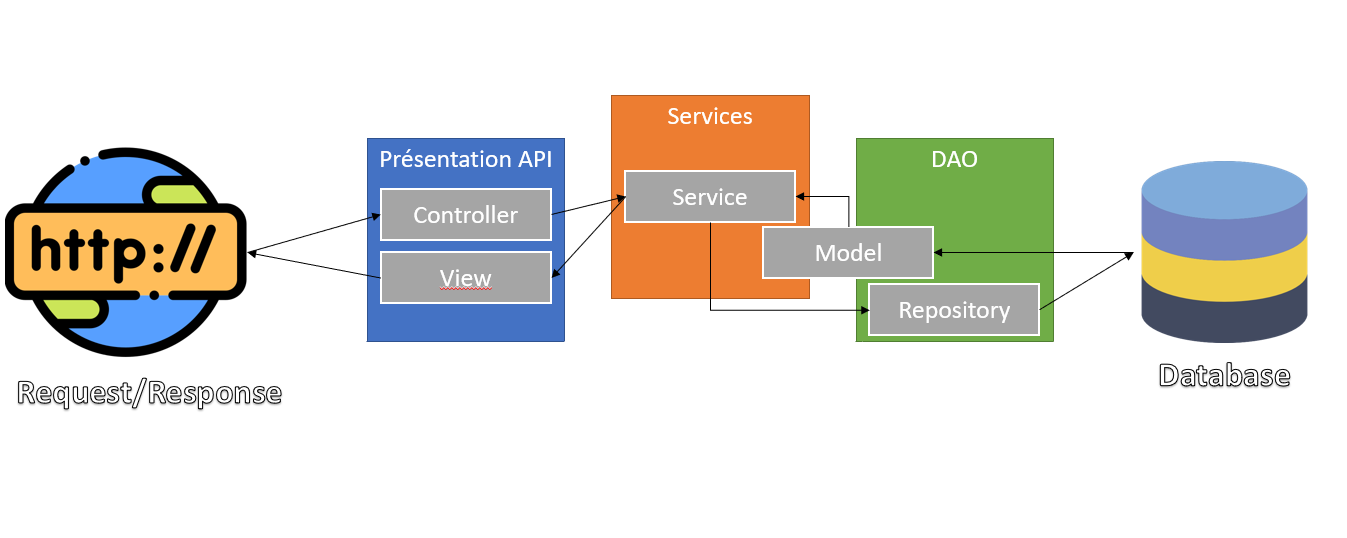
\includegraphics[width=\textwidth]{Figures/back.PNG}}
	\caption{\label{fig:my-label} Architecture applicative backend}
\end{figure}

\subsubsection{Cas g\'en\'eral pour le backoffice}

L'architecture qu'on va utiliser agit comme un conteneur d'\'etat et facilite la gestion du flux de donn\'ees de notre application. Il a \'et\'e introduit en 2015 lors de la conf\'erence \textcolor{red}{ReactEurope} de \textcolor{red}{Dan Abramov}. Elle ressemble \`a l'architecture Flux et a beaucoup en commun avec elle.

\begin{figure}[H]
	\center{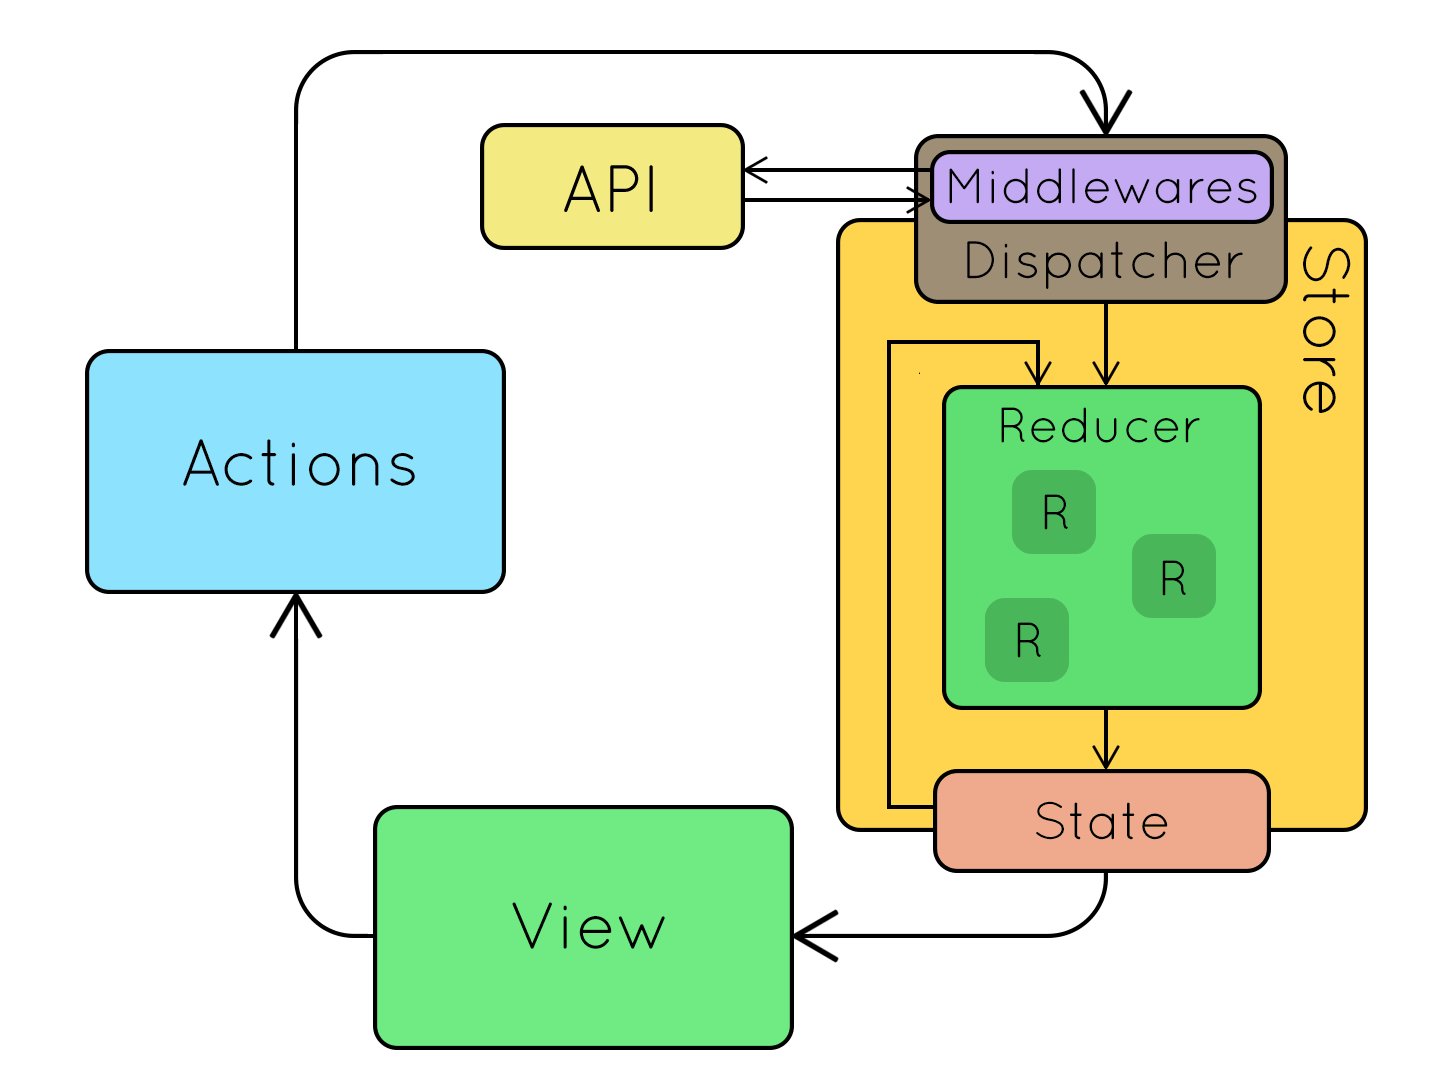
\includegraphics[width=0.6\textwidth]{Figures/backoffice.png}}
	\caption{\label{fig:my-label} Architecture Applicative backoffice}
\end{figure}

Nous avons les composants de vue qui envoient une action. La m\^eme action peut \^etre envoy\'ee par une autre partie de notre syst\`eme. Cette action est envoy\'ee non pas \`a un hub central, mais directement au store. Nous disons "store" et non "stores" car il n'y en a qu'un global. La logique qui a d\'ecid\'e comment nos donn\'ees changent vit dans des fonctions pures appel\'ees reducers. Une fois que le store re\c{c}oit une action, il demande aux reducers la nouvelle version de l'\'etat en envoyant l'\'etat actuel et l'action en question. Ensuite, de mani\`ere immuable, le reducer doit retourner le nouvel \'etat. Le store continue \`a partir de l\`a et met \`a jour son \'etat interne. Enfin, le composant c\^abl\'e au store est rendu \`a nouveau.


\subsubsection{Cas g\'en\'eral pour le frontoffice}

Le mod\'ele de conception architecturale \gls{MVP1} est un mod\'ele de conception assez connu des d\'eveloppeurs Android. Il vous permet de d\'ecoupler la logique m\'etier de la logique de vue (Activit\'e / Fragment) en introduisant un interm\'ediaire appel\'e Pr\'esentateur.

Comme son nom l'indique, \gls{MVP1} est divis\'e en trois couches diff\'erentes.

\begin{figure}[H]
	\center{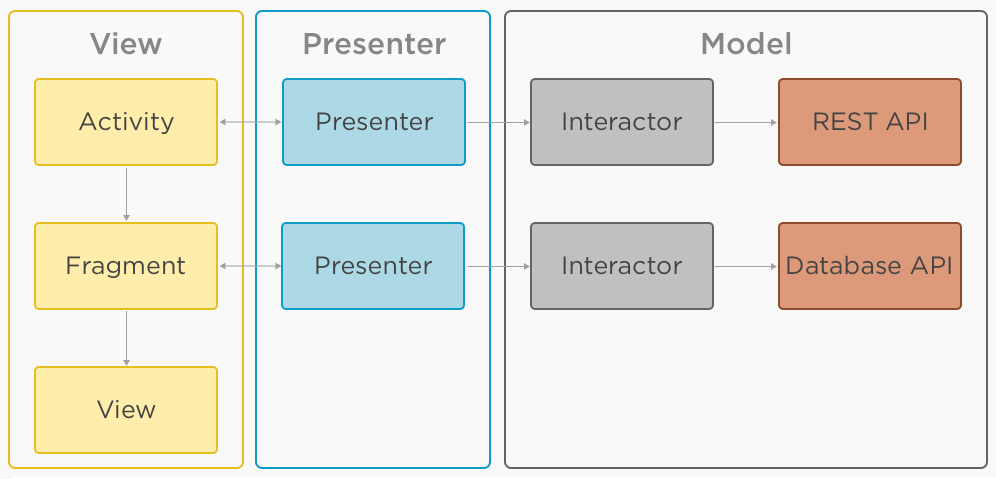
\includegraphics[width=\textwidth]{Figures/frontoffice.PNG}}
	\caption{\label{fig:my-label} Architecture Applicative frontoffice}
\end{figure}

\begin{itemize}

\item \textbf{Mod\'ele} - Comme mentionn\'e ci-dessous, o\`u est stock\'ee votre logique m\'etier et votre application de donn\'ees? Sous Android, le r\^ole d'un mod\'ele est g\'en\'eralement jou\'e par l'\gls{API} ou l'\gls{API} \gls{REST}.

Il est non seulement responsable du stockage des donn\'ees de l'application, mais \'egalement de composants contenant des responsabilit\'es pour la g\'en\'eration, l'exposition et la r\'ecup\'eration des donn\'ees.

En g\'en\'eral, toutes ces fonctionnalit\'es sont ex\'ecut\'ees en arri\'ere-plan car elles peuvent bloquer le thread d'interface utilisateur.

\item \textbf{View} - View est essentiellement une interface d'utilisateur passive qui est responsable du routage de l'action de l'utilisateur vers le pr\'esentateur. 

En g\'en\'eral, l'affichage n'est pas visible pour votre mod\'ele, \`a l'exception du POJOS et des entit\'es de l'application. Pour faire plus simplement, les vues ne communiquent pas directement avec les mod\'eles. Cependant, ils parlent aux pr\'esentateurs.

\item \textbf{Presenter} - Le pr\'esentateur est l'interm\'ediaire ou le m\'ediateur entre View et Model.

En termes g\'en\'eraux, Presenter interroge le mod\'ele et met \`a jour la vue tout en r\'epondant aux interactions de l'utilisateur.

Il surveille la fa\c{c}on dont ils sont, et ils ne peuvent pas le g\'erer.

\end{itemize}

\subsubsection{Les services externes}

Dans notre projet, on est besoin de trois services externes qui sont d\'ej\`a r\'ealiser par l'entit\'e \gls{DF}. La communication avec ces services se base sur les requ\^etes \gls{HTTP} \& leurs utilit\'es sont:
\begin{itemize}
\item \textbf{Service d'authentification} : permet de v\'erifier l'identit\'e d'un utilisateur, est ce qu'il est appartient au groupe \gls{OCP}.
\item \textbf{Service Minio} : permet de stocker les fichiers de grandes tailles, dans notre cas, on veut stocker les attachements des anomalies. On va utiliser le protocole \gls{NFS} comme protocole lors du stockage pour accéder \`a notre réseau \`a nos fichiers distants.
\item \textbf{Service Notification} : permet d'envoyer des e-mails et des messages \gls{SMS}.
\end{itemize}


\section{Entity relationship diagram}
Un certain nombre de techniques de mod\'elisation de donnd\'ees sont utilisd\'ees aujourd'hui. L'un des plus courants est le diagramme de relation d'entitd\'e (\gls{ERD}). Plusieurs notations \gls{ERD} sont disponibles. Nous avons utilis\'e la notation du Crow's Foot.

La \textbf{cardinalit\'e} et la \textbf{modalit\'e} sont les indicateurs des r\`egles de gestion entourant une relation. La cardinalit\'e fait r\'ef\'erence au nombre maximum de fois qu'une instance d'une entit\'e peut \^etre associ\'ee \`a des instances de l'entit\'e associ\'ee. La modalit\'e fait r\'ef\'erence au nombre minimum de fois qu'une instance d'une entit\'e peut \^etre associ\'ee \`a une instance de l'entit\'e associ\'ee.

\begin{table}[H]
\begin{center}
\begin{tabular}{ |l|l| }
\hline Symbole & cardinalit\'e \\ \hline \hline
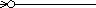
\includegraphics[width=0.2\textwidth]{Figures/0+.png}
& z\'ero ou plus \\ \hline
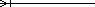
\includegraphics[width=0.2\textwidth]{Figures/1+.png}
& 1 ou plus \\ \hline
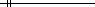
\includegraphics[width=0.2\textwidth]{Figures/11.png}
& 1 et seulement 1 \\ \hline
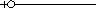
\includegraphics[width=0.2\textwidth]{Figures/01.png}
& z\'ero ou 1 \\
\hline
\end{tabular}
\caption{Cardinalit\'e du Crow's Foot}
\end{center}
\end{table}

Le diagramme du crow's foot de notre projet prospektor est repr\'esent\'e dans le figure ci-dessous :

\begin{figure}[H]
	\center{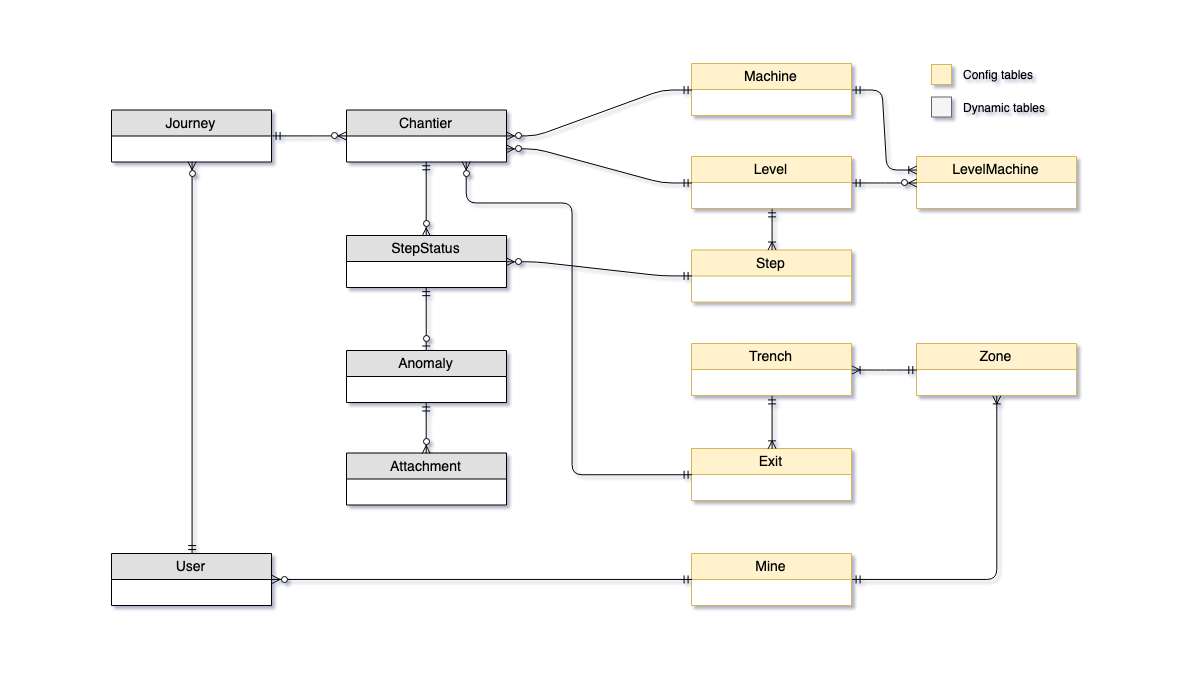
\includegraphics[width=\textwidth]{Figures/crowsfeet.PNG}}
	\caption{\label{fig:my-label} Diagramme de Crow's Foot}
\end{figure}

Cette diapositive repr\'esente le diagramme des entit\'es qui sont utilises dans notre projet. Elles sont composes \`a deux types :
\begin{itemize}
\item \textbf{Statique} : repr\'esenter par la couleur jaune, contient des informations statiques sur les entit\'es de g\'eolocalisation (Mine, Zone, Tranch\'ee, Sorties), les machines existantes et les phases d'extraction de phosphates.
\item \textbf{Dynamique} : repr\'esenter par la couleur gris, contient des informations dynamiques et changeable, par exemple : les utilisateurs, les anomalies, les attachements, les chantiers visites ainsi les tourn\'ees de chaque exploitants.
\end{itemize}

Dans la figure ci-dessous 

\section{Conclusion}

Dans ce chapitre nous avons entam\'e la conception g\'en\'erale du projet en d\'ecrivant l'architechture du projet de mani\`ere d\'etaill\'ee. Pour les technologies utilises et les outils de d\'eveloppements, on va les pr\'esenter dans le prochaine chapitre.

